\documentclass[12pt]{article}
\usepackage{fullpage,graphicx,psfrag,amsmath,amsfonts,verbatim}
\usepackage[small,bf]{caption}
\usepackage{float}

\input defs.tex

\bibliographystyle{alpha}

\title{Assignment 4 CME 241}
\author{Taylor Howell}

\begin{document}
\maketitle

\newpage
\section{Manual value iteration}
\begin{figure}[!htb]
	\centering
	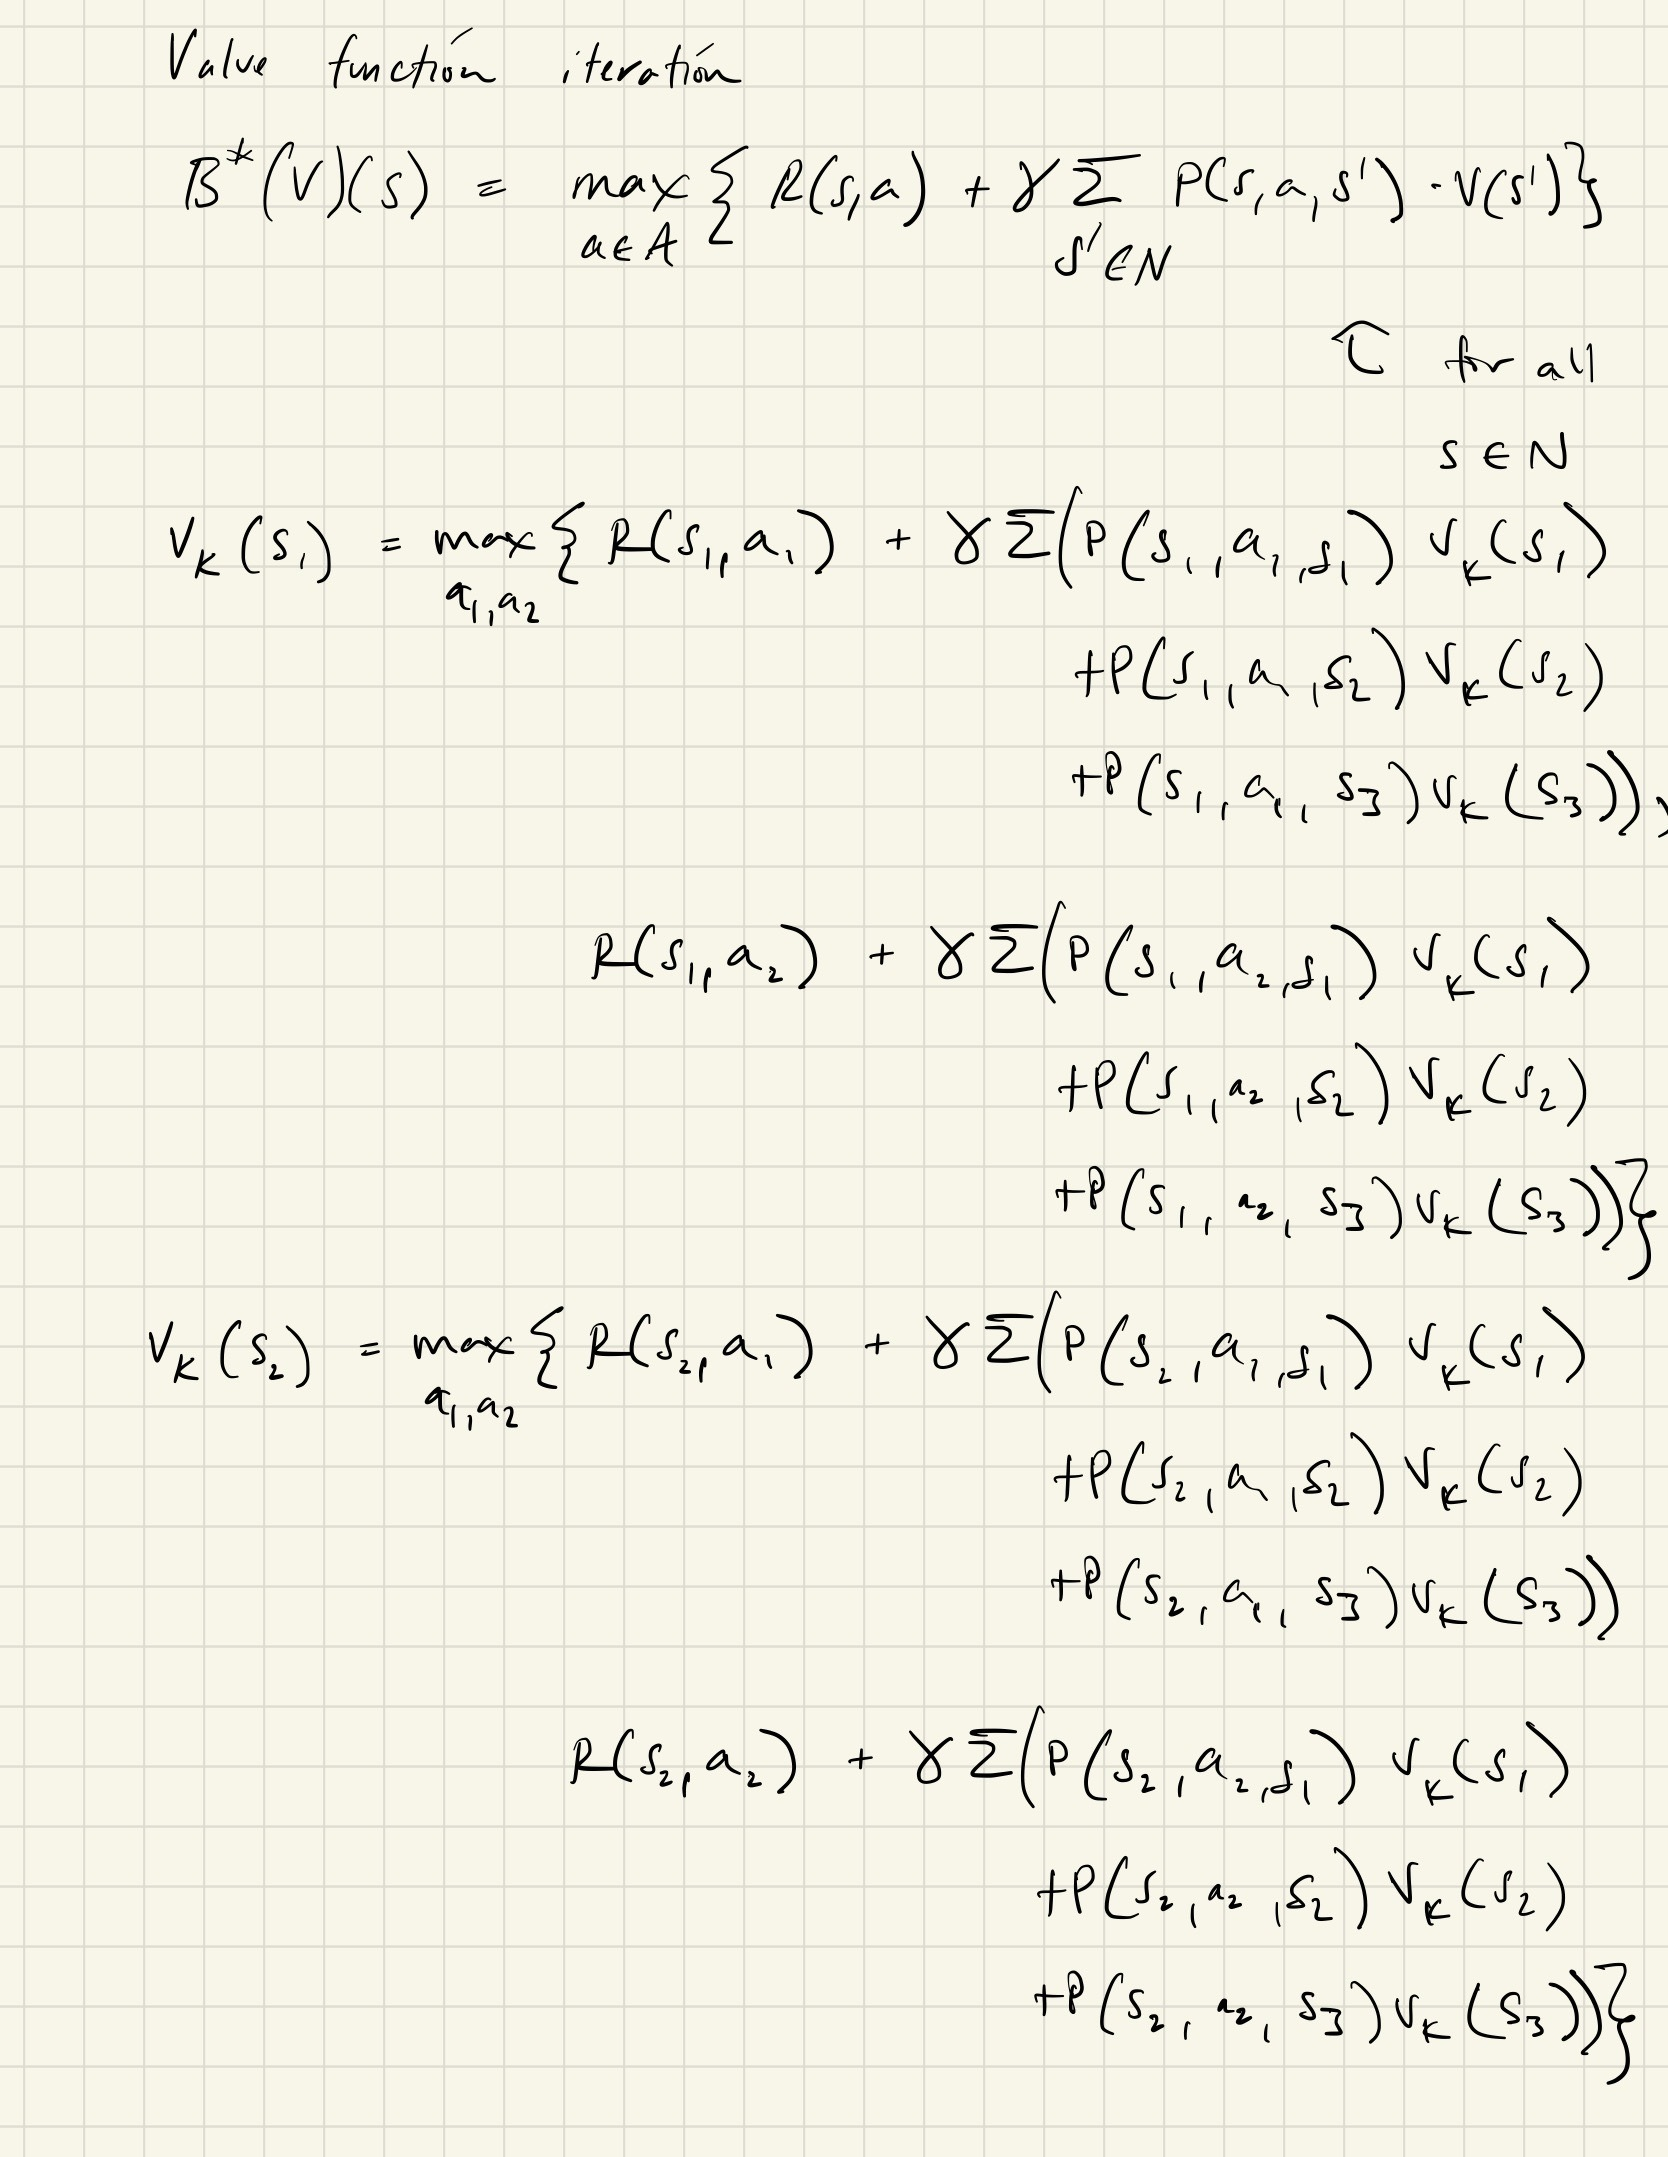
\includegraphics[width=.75\textwidth]{ipad/q1_1.jpg}
\end{figure}

\begin{figure}[!htb]
	\centering
	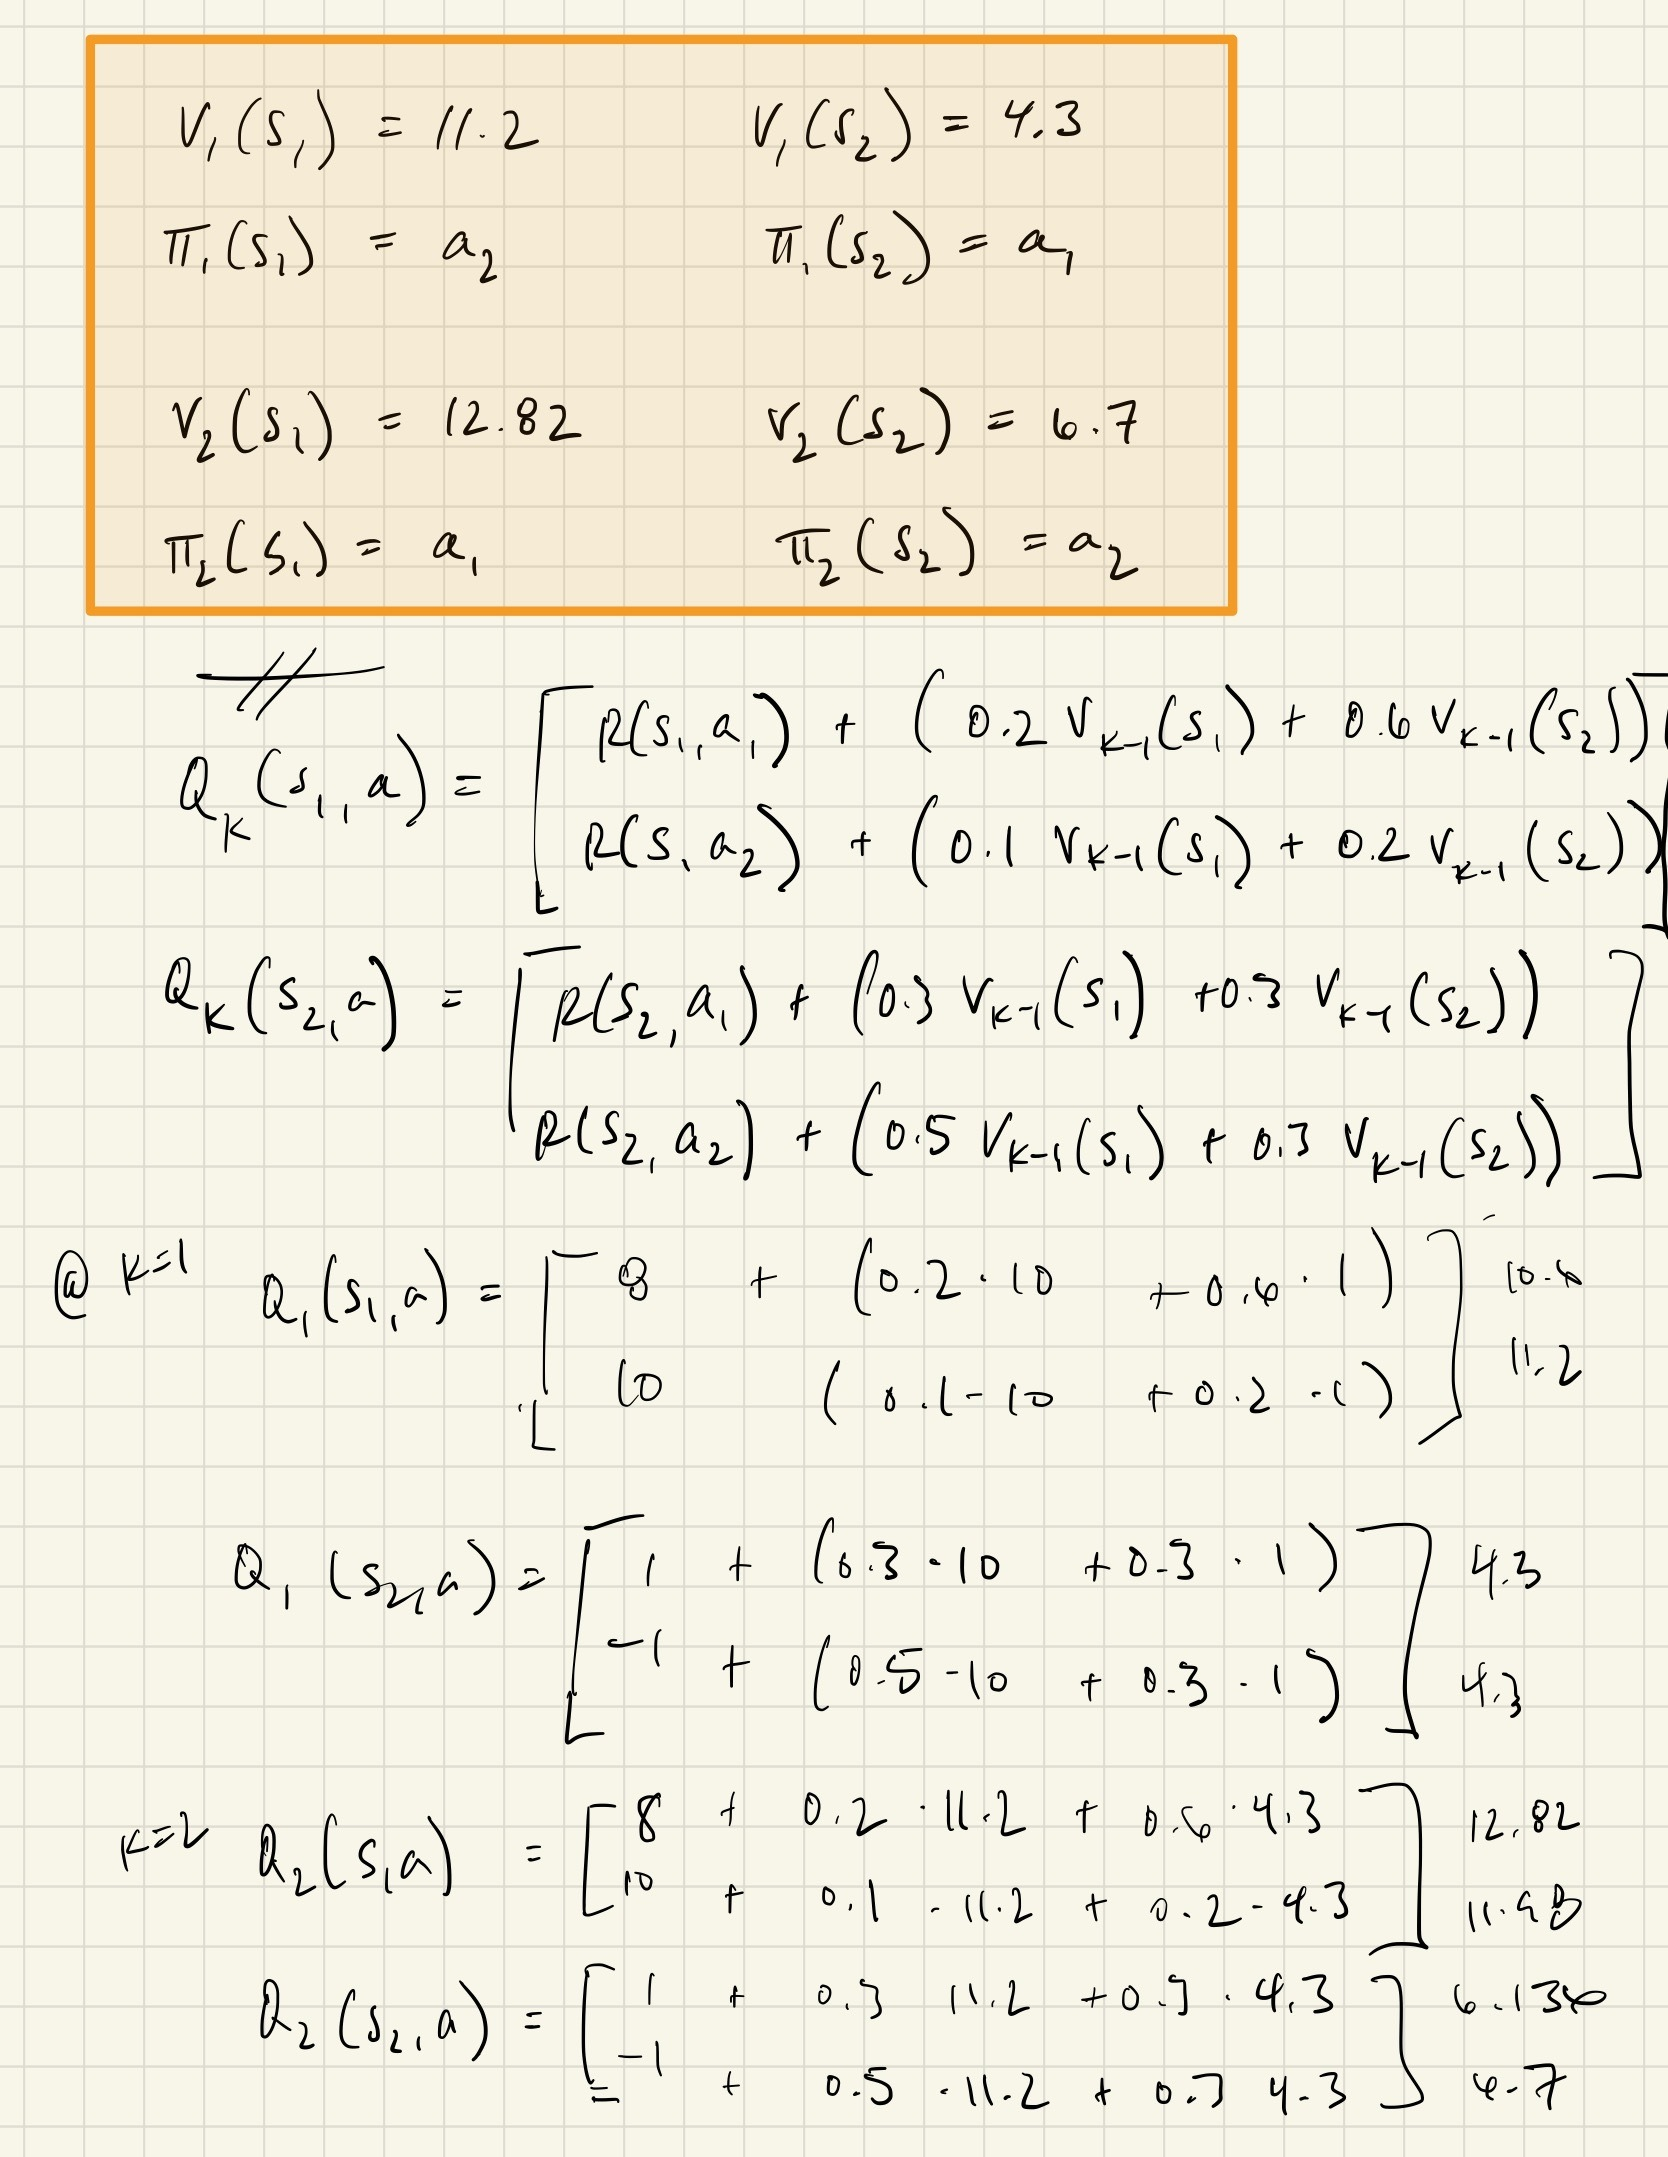
\includegraphics[width=.75\textwidth]{ipad/q1_2.jpg}
\end{figure}

\begin{figure}[!htb]
	\centering
	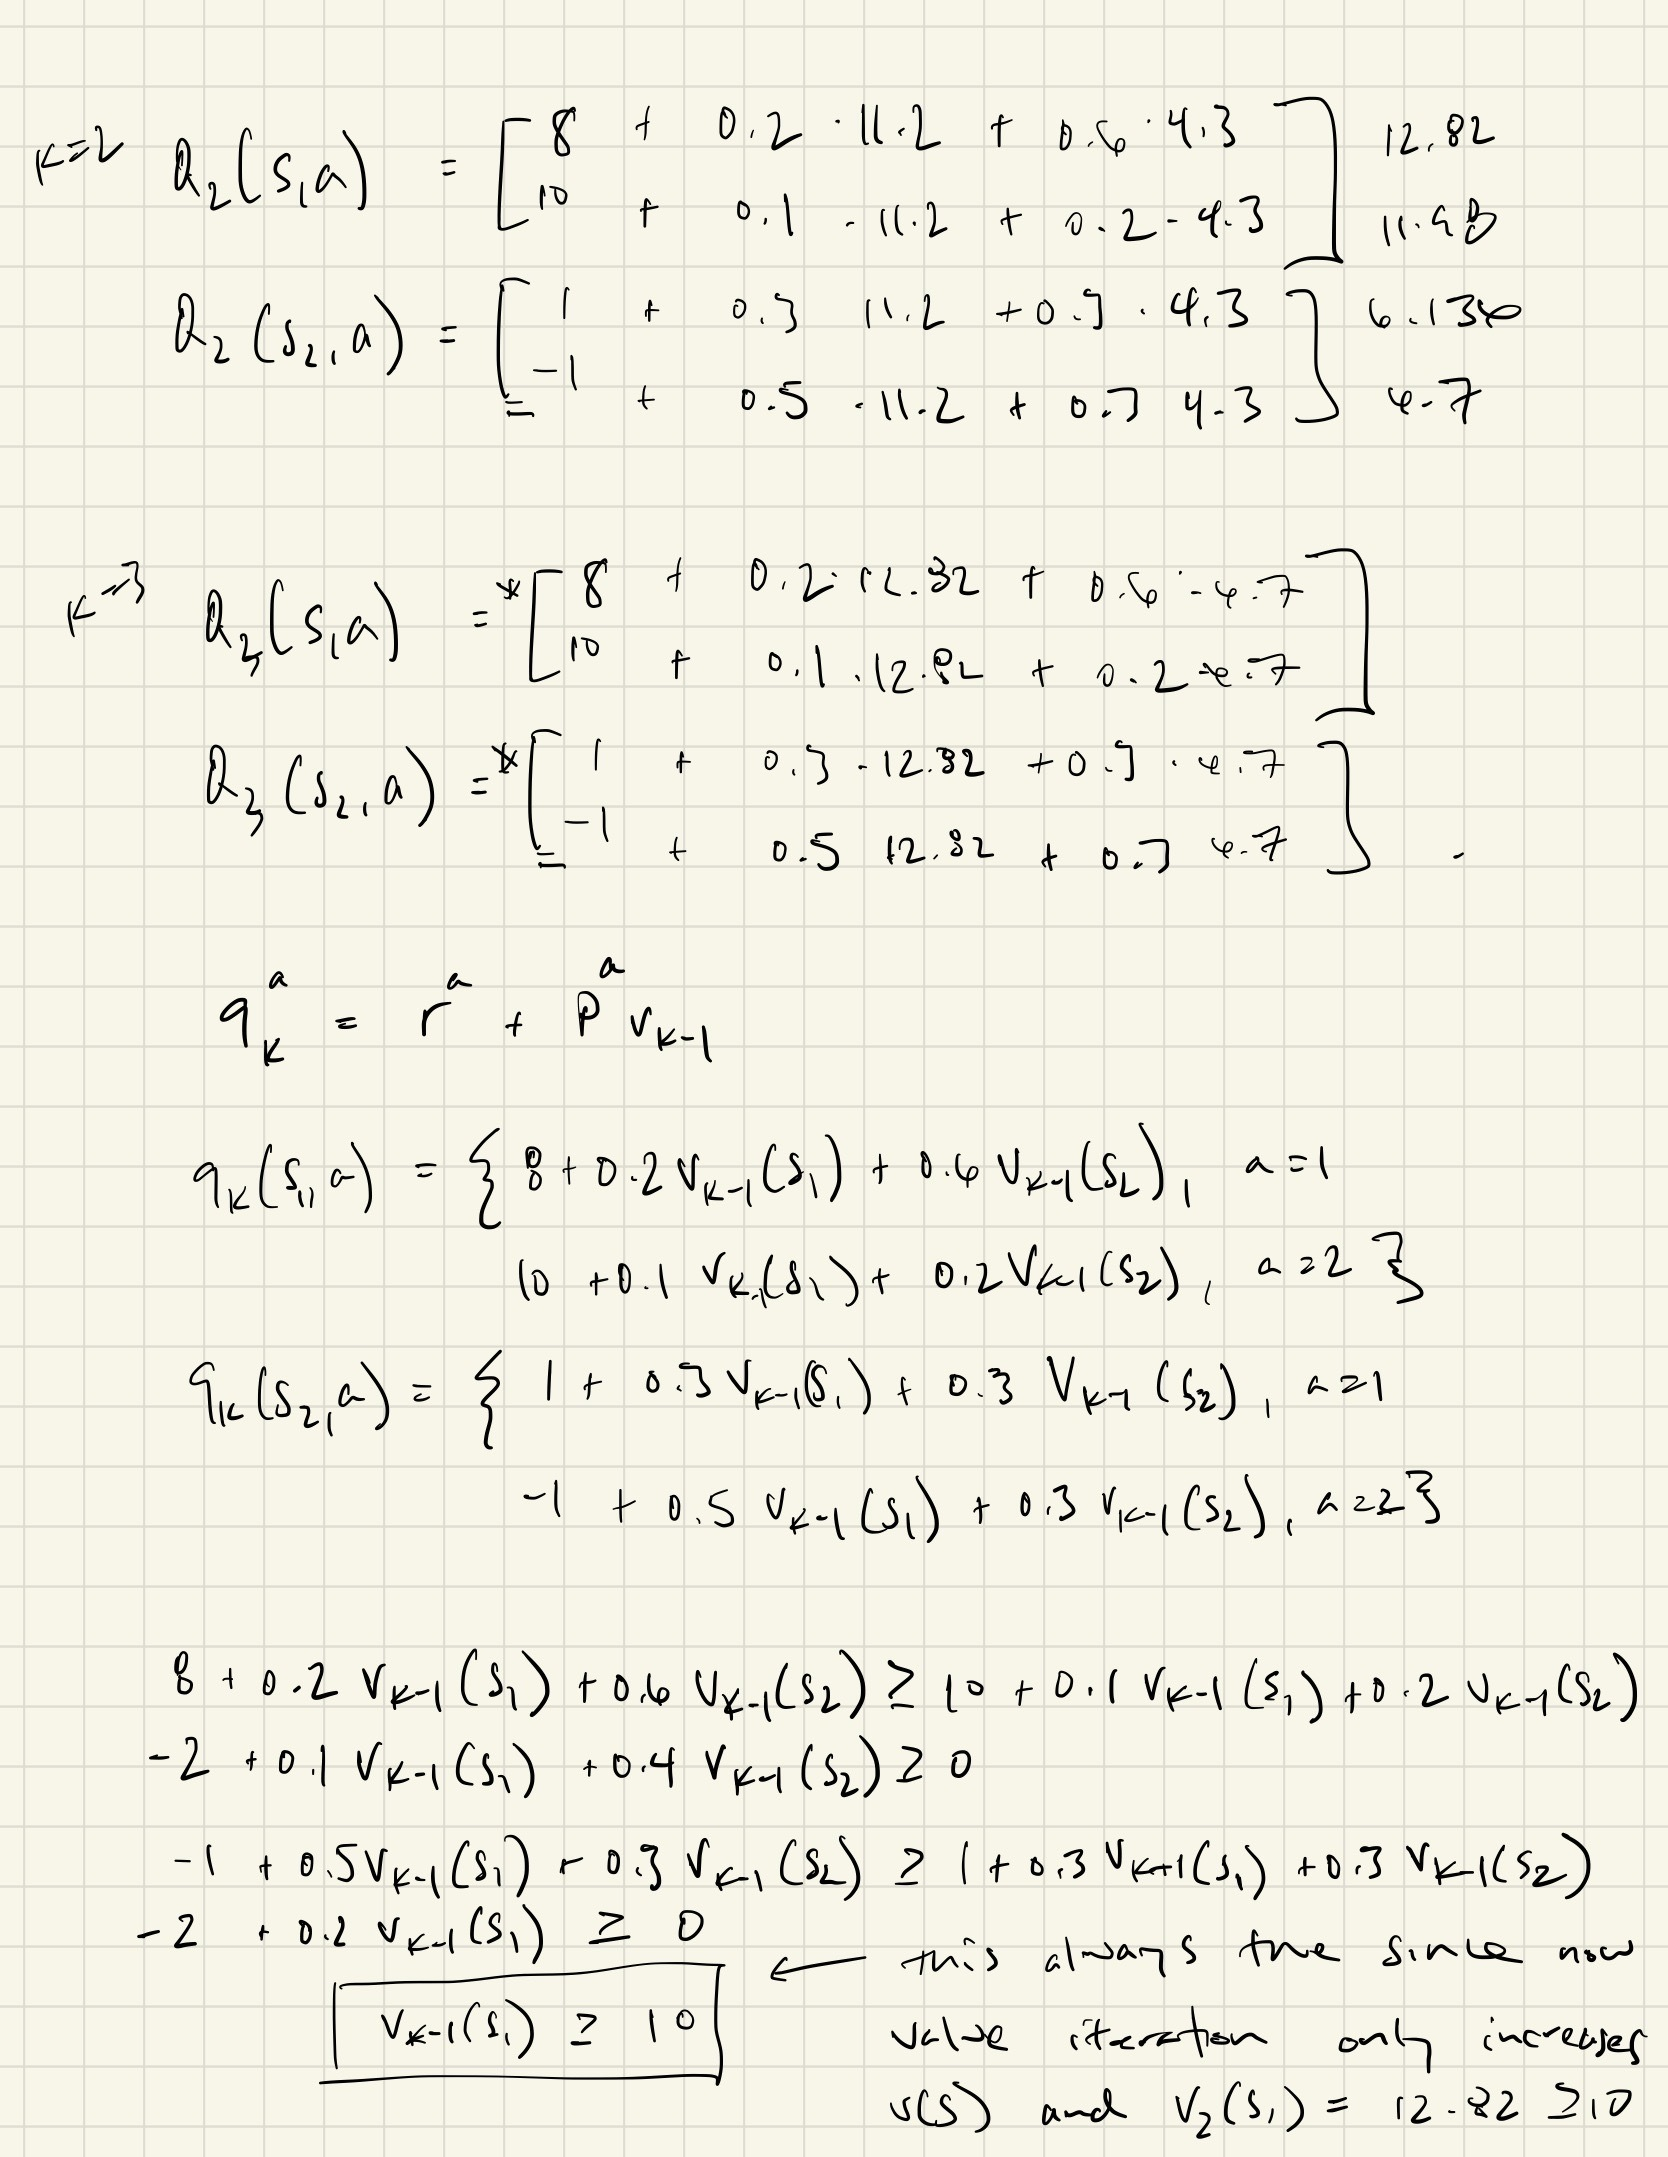
\includegraphics[width=.75\textwidth]{ipad/q1_3.jpg}
\end{figure}

\begin{figure}[!htb]
	\centering
	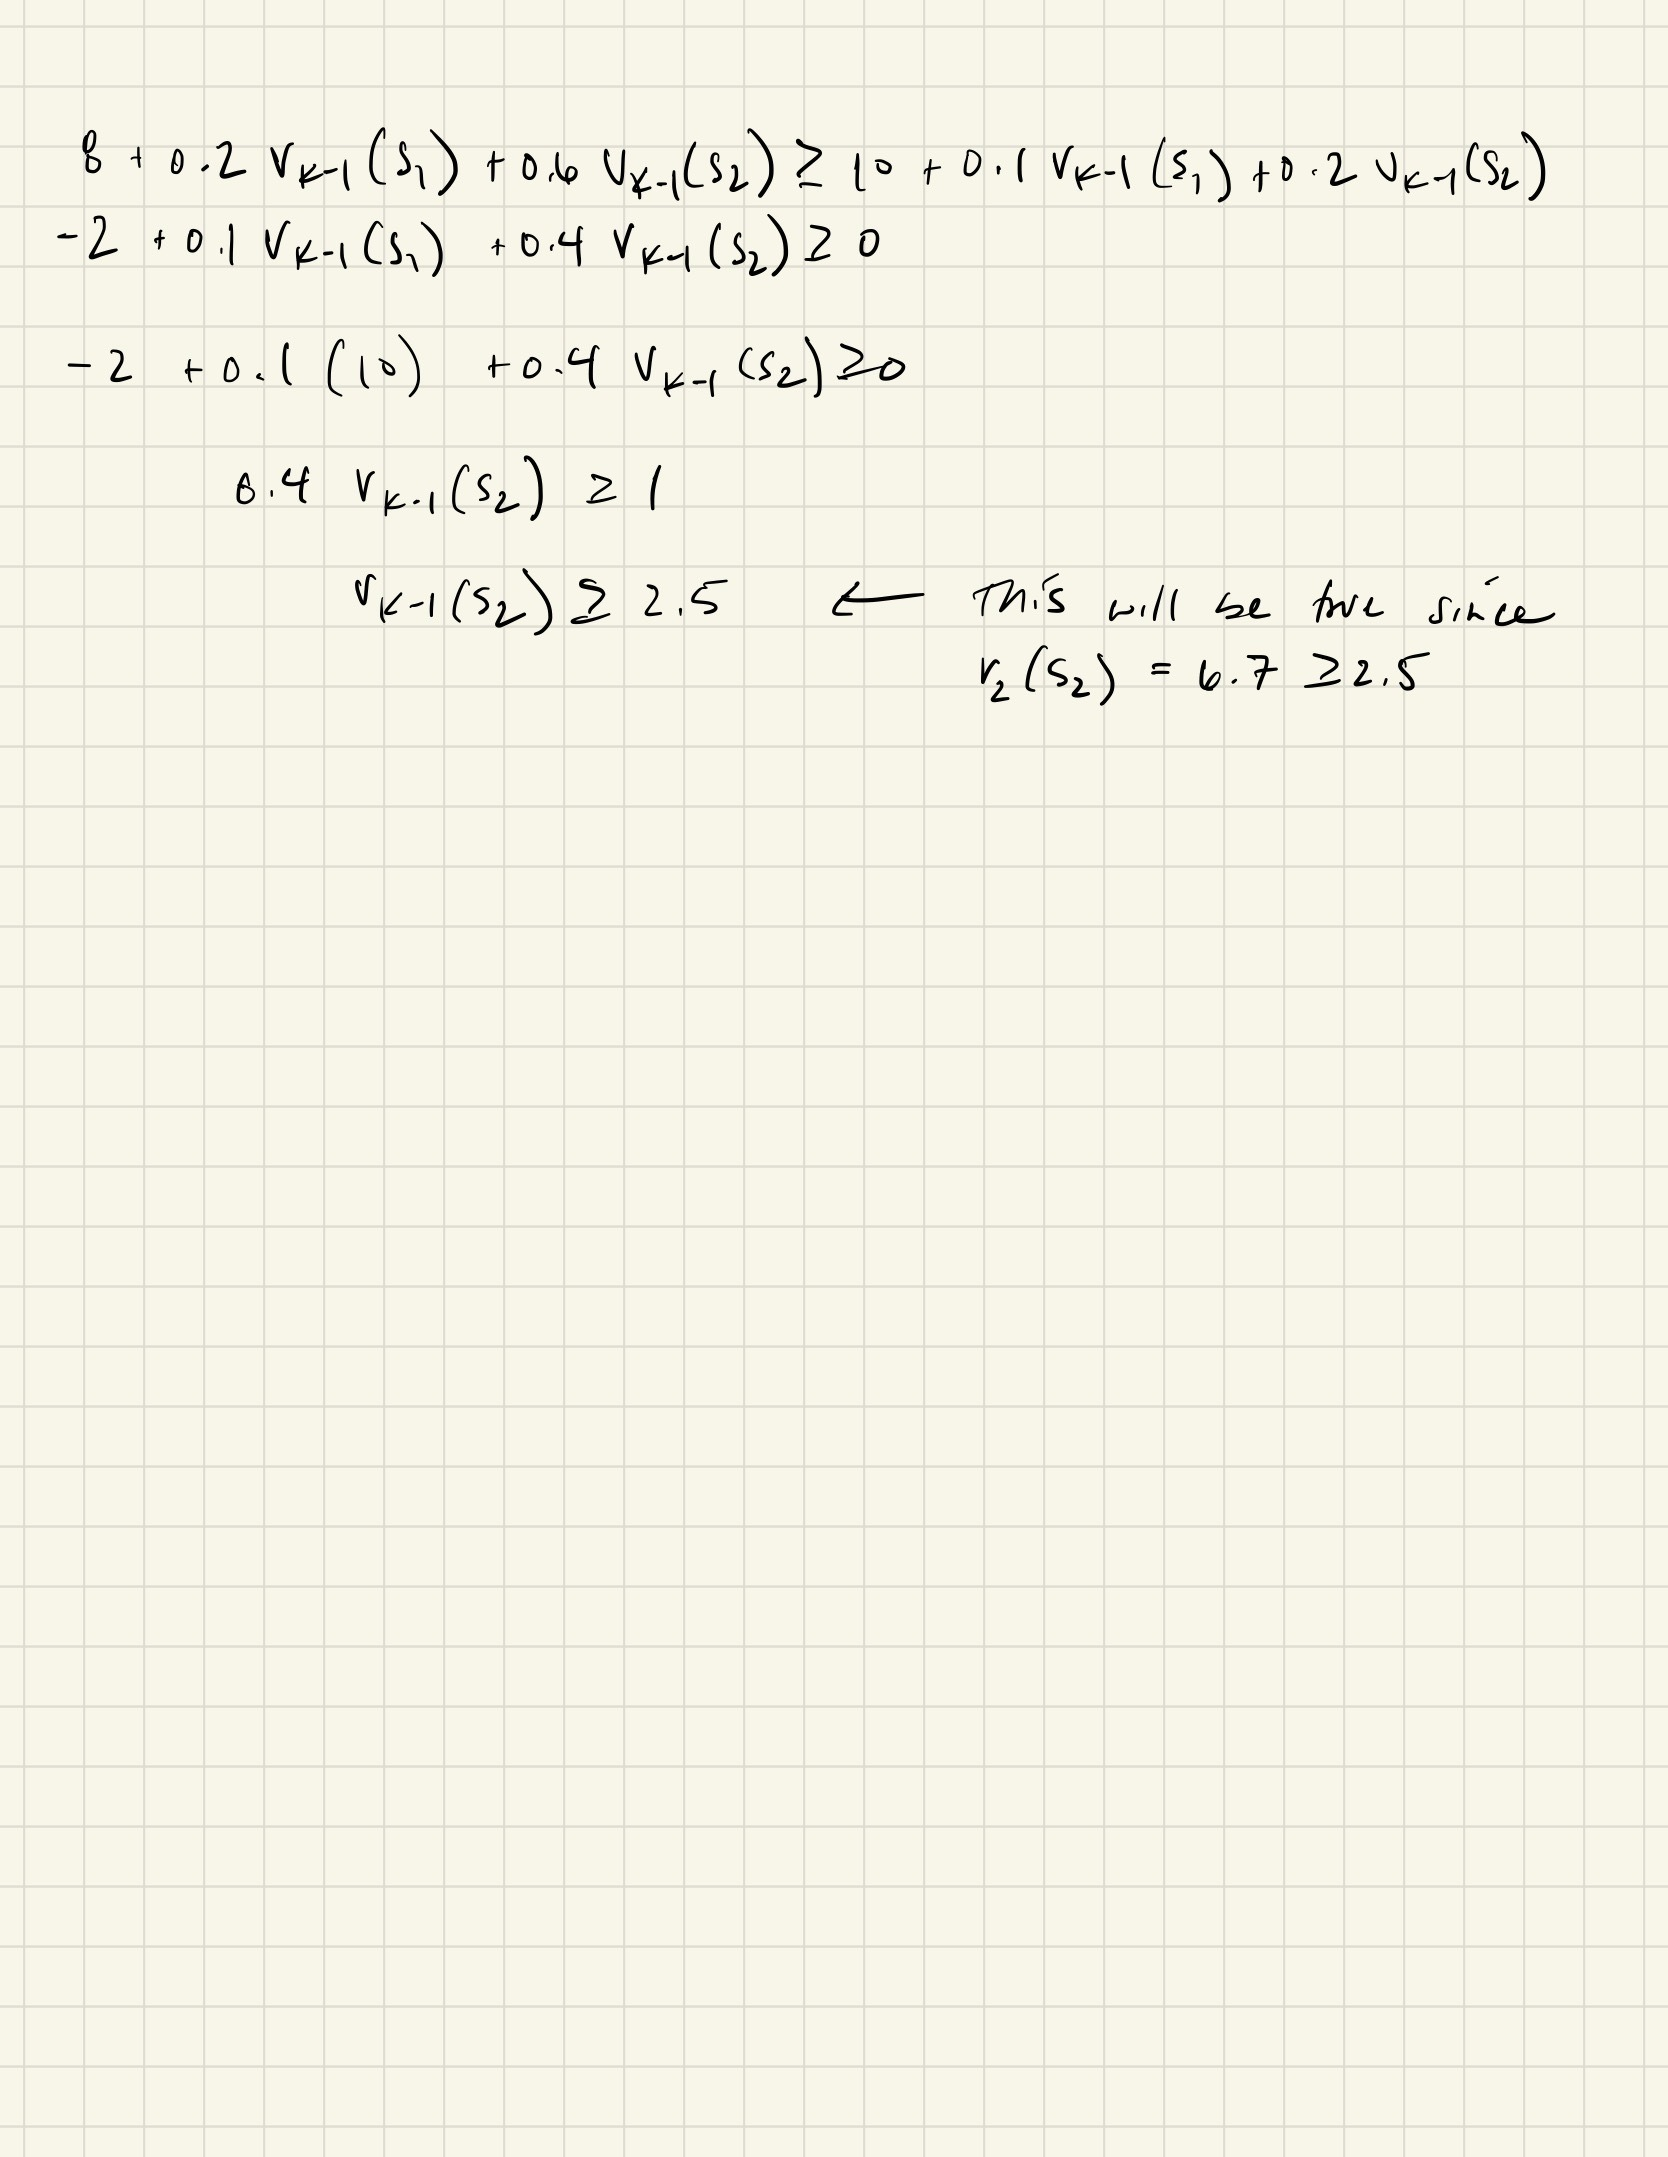
\includegraphics[width=.75\textwidth]{ipad/q1_4.jpg}
\end{figure}

\clearpage
\section{Frog croaking revisited}
For this problem, I have reimplemented my MDP in Julia (see \texttt{frog\_escape.jl}). Additionally, I have implemented value iteration (\texttt{value\_iteration.jl}) and policy iteration (\texttt{policy\_iteration.jl}) from scratch.

I also remodeled the reward function since the last assignment:
$$\mathcal{R}(s, a) = 1 \cdot \mathcal{P}(S_t = s, A_t = a, S_{t+1} = n)$$

%\begin{figure}
%	\centering
%	\includegraphics[width=.5\textwidth]{}
%\end{figure}

\section{Job-hopping and wages-utility-maximization}
I model the MDP under two different assumptions. First, I model the offered job as random (i.e., you choose to select the job or not without knowing which job you are offered), see Fig. \ref{fig:q3_1}. Second, I model the problem assuming the offered job is known before the decision whether to accept or reject must be made, see Fig. \ref{fig:q3_2}. I implement the MDP in Julia (\texttt{q3\_job\_hopping.jl}) and wrote an implementation of value iteration that is custom to this problem.

\begin{figure}[h]
	\centering
	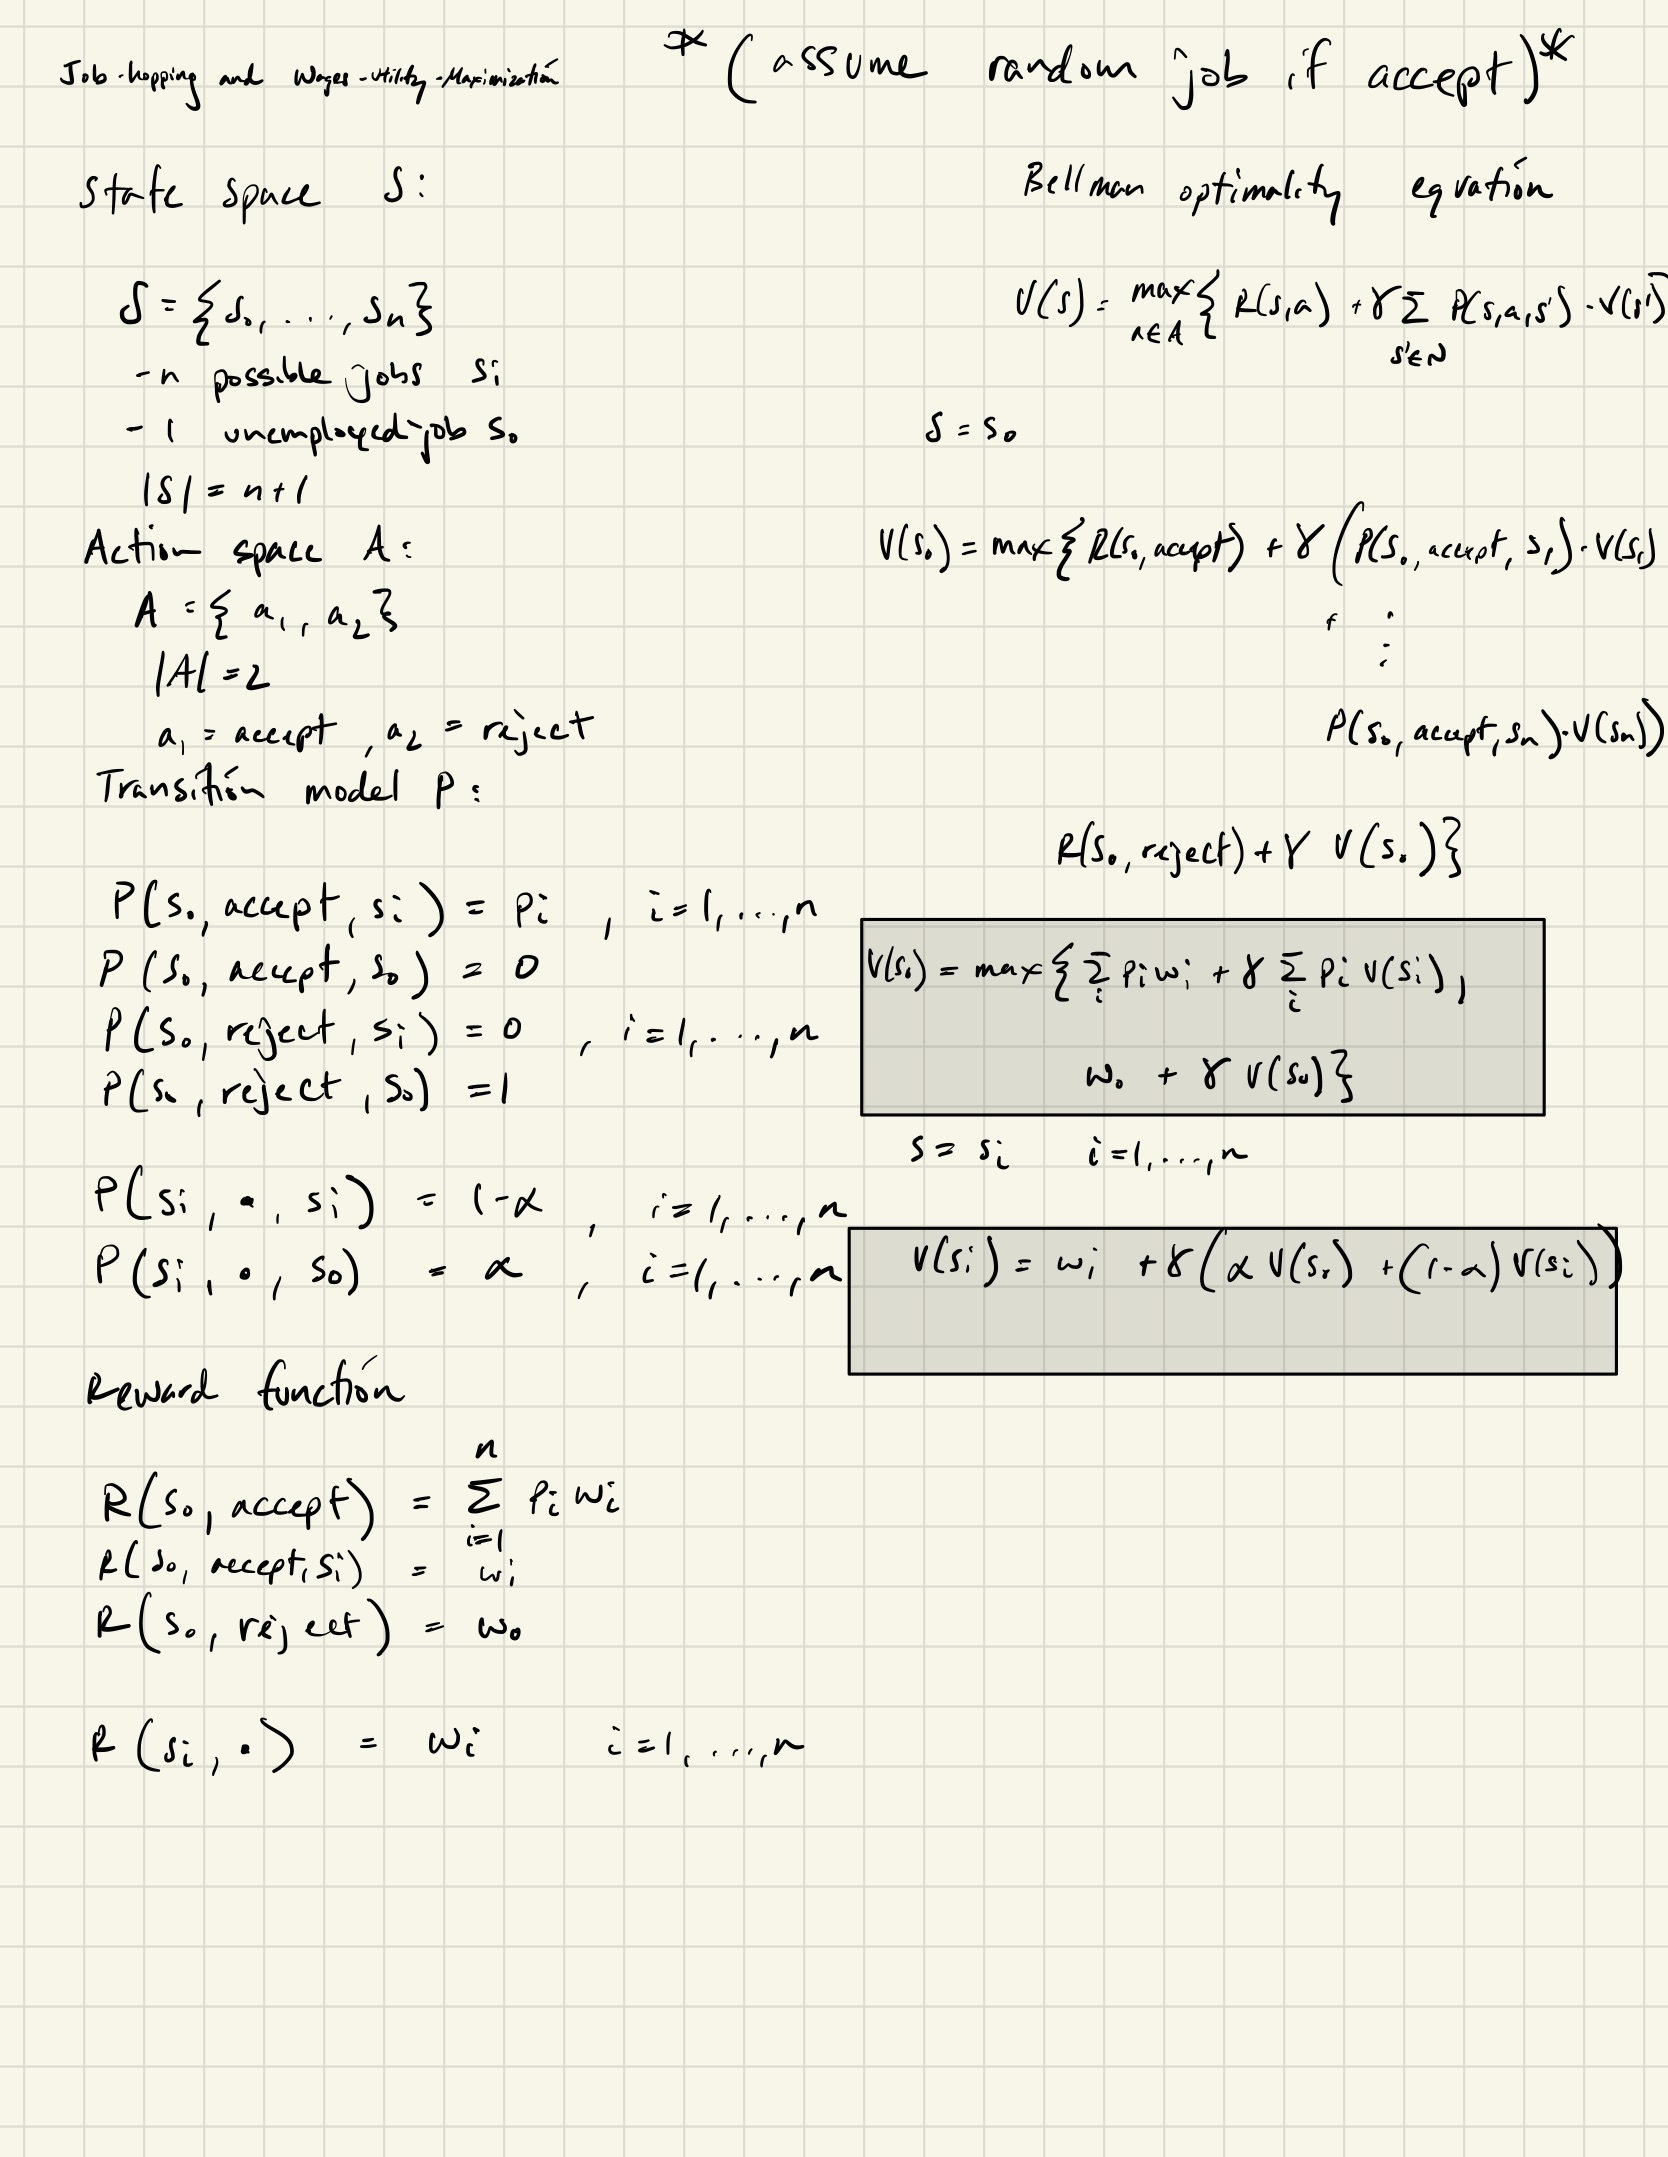
\includegraphics[width=.75\textwidth]{ipad/q3_1.jpg}
	\caption{Job-hopping MDP random next job.}
	\label{fig:q3_1}
\end{figure}

\begin{figure}[h]
	\centering
	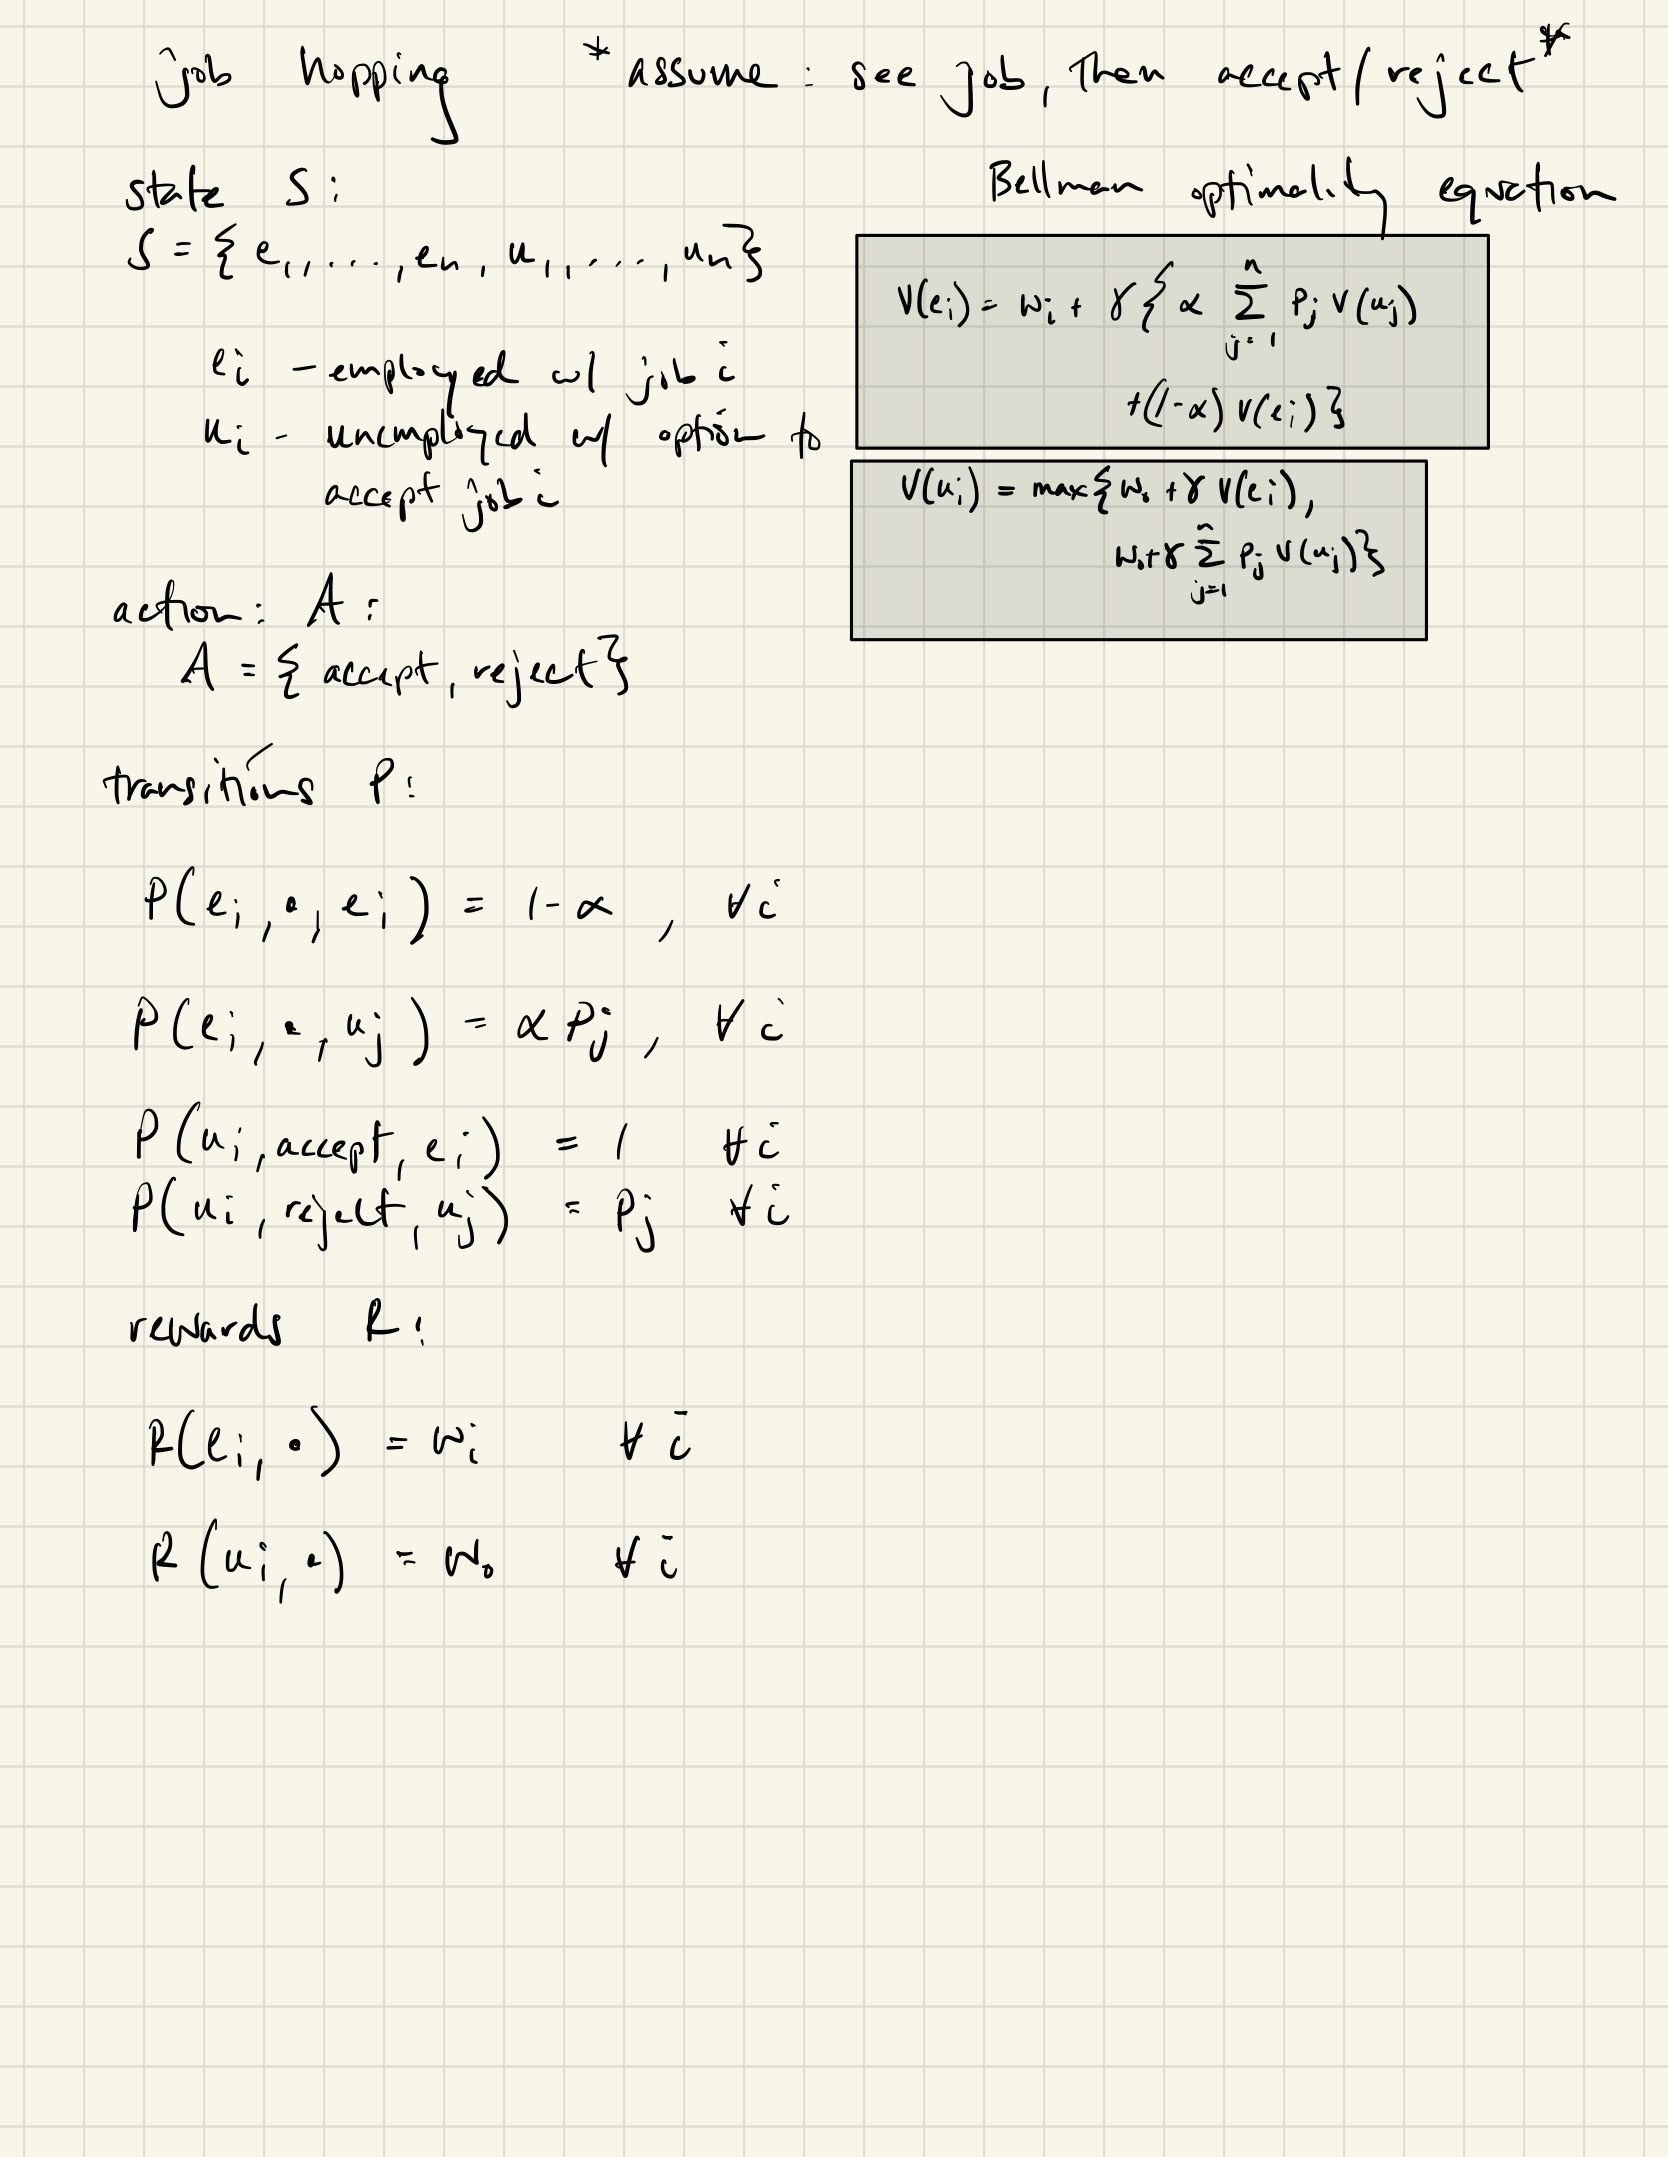
\includegraphics[width=.75\textwidth]{ipad/q3_2.jpg}
	\caption{Job-hopping MDP known next job.}
	\label{fig:q3_2}
\end{figure}

\section{Two-Stores Inventory Control}

I first implement the simple inventory problem for a single store in Julia \texttt{q4\_simple\_inventory.jl} and then implement the two-store problem \texttt{q4\_two\_store\_inventory.jl}. My MDP formulation for the two-store problem is show in Fig. \ref{fig:q4}.

\begin{figure}[h]
	\centering
	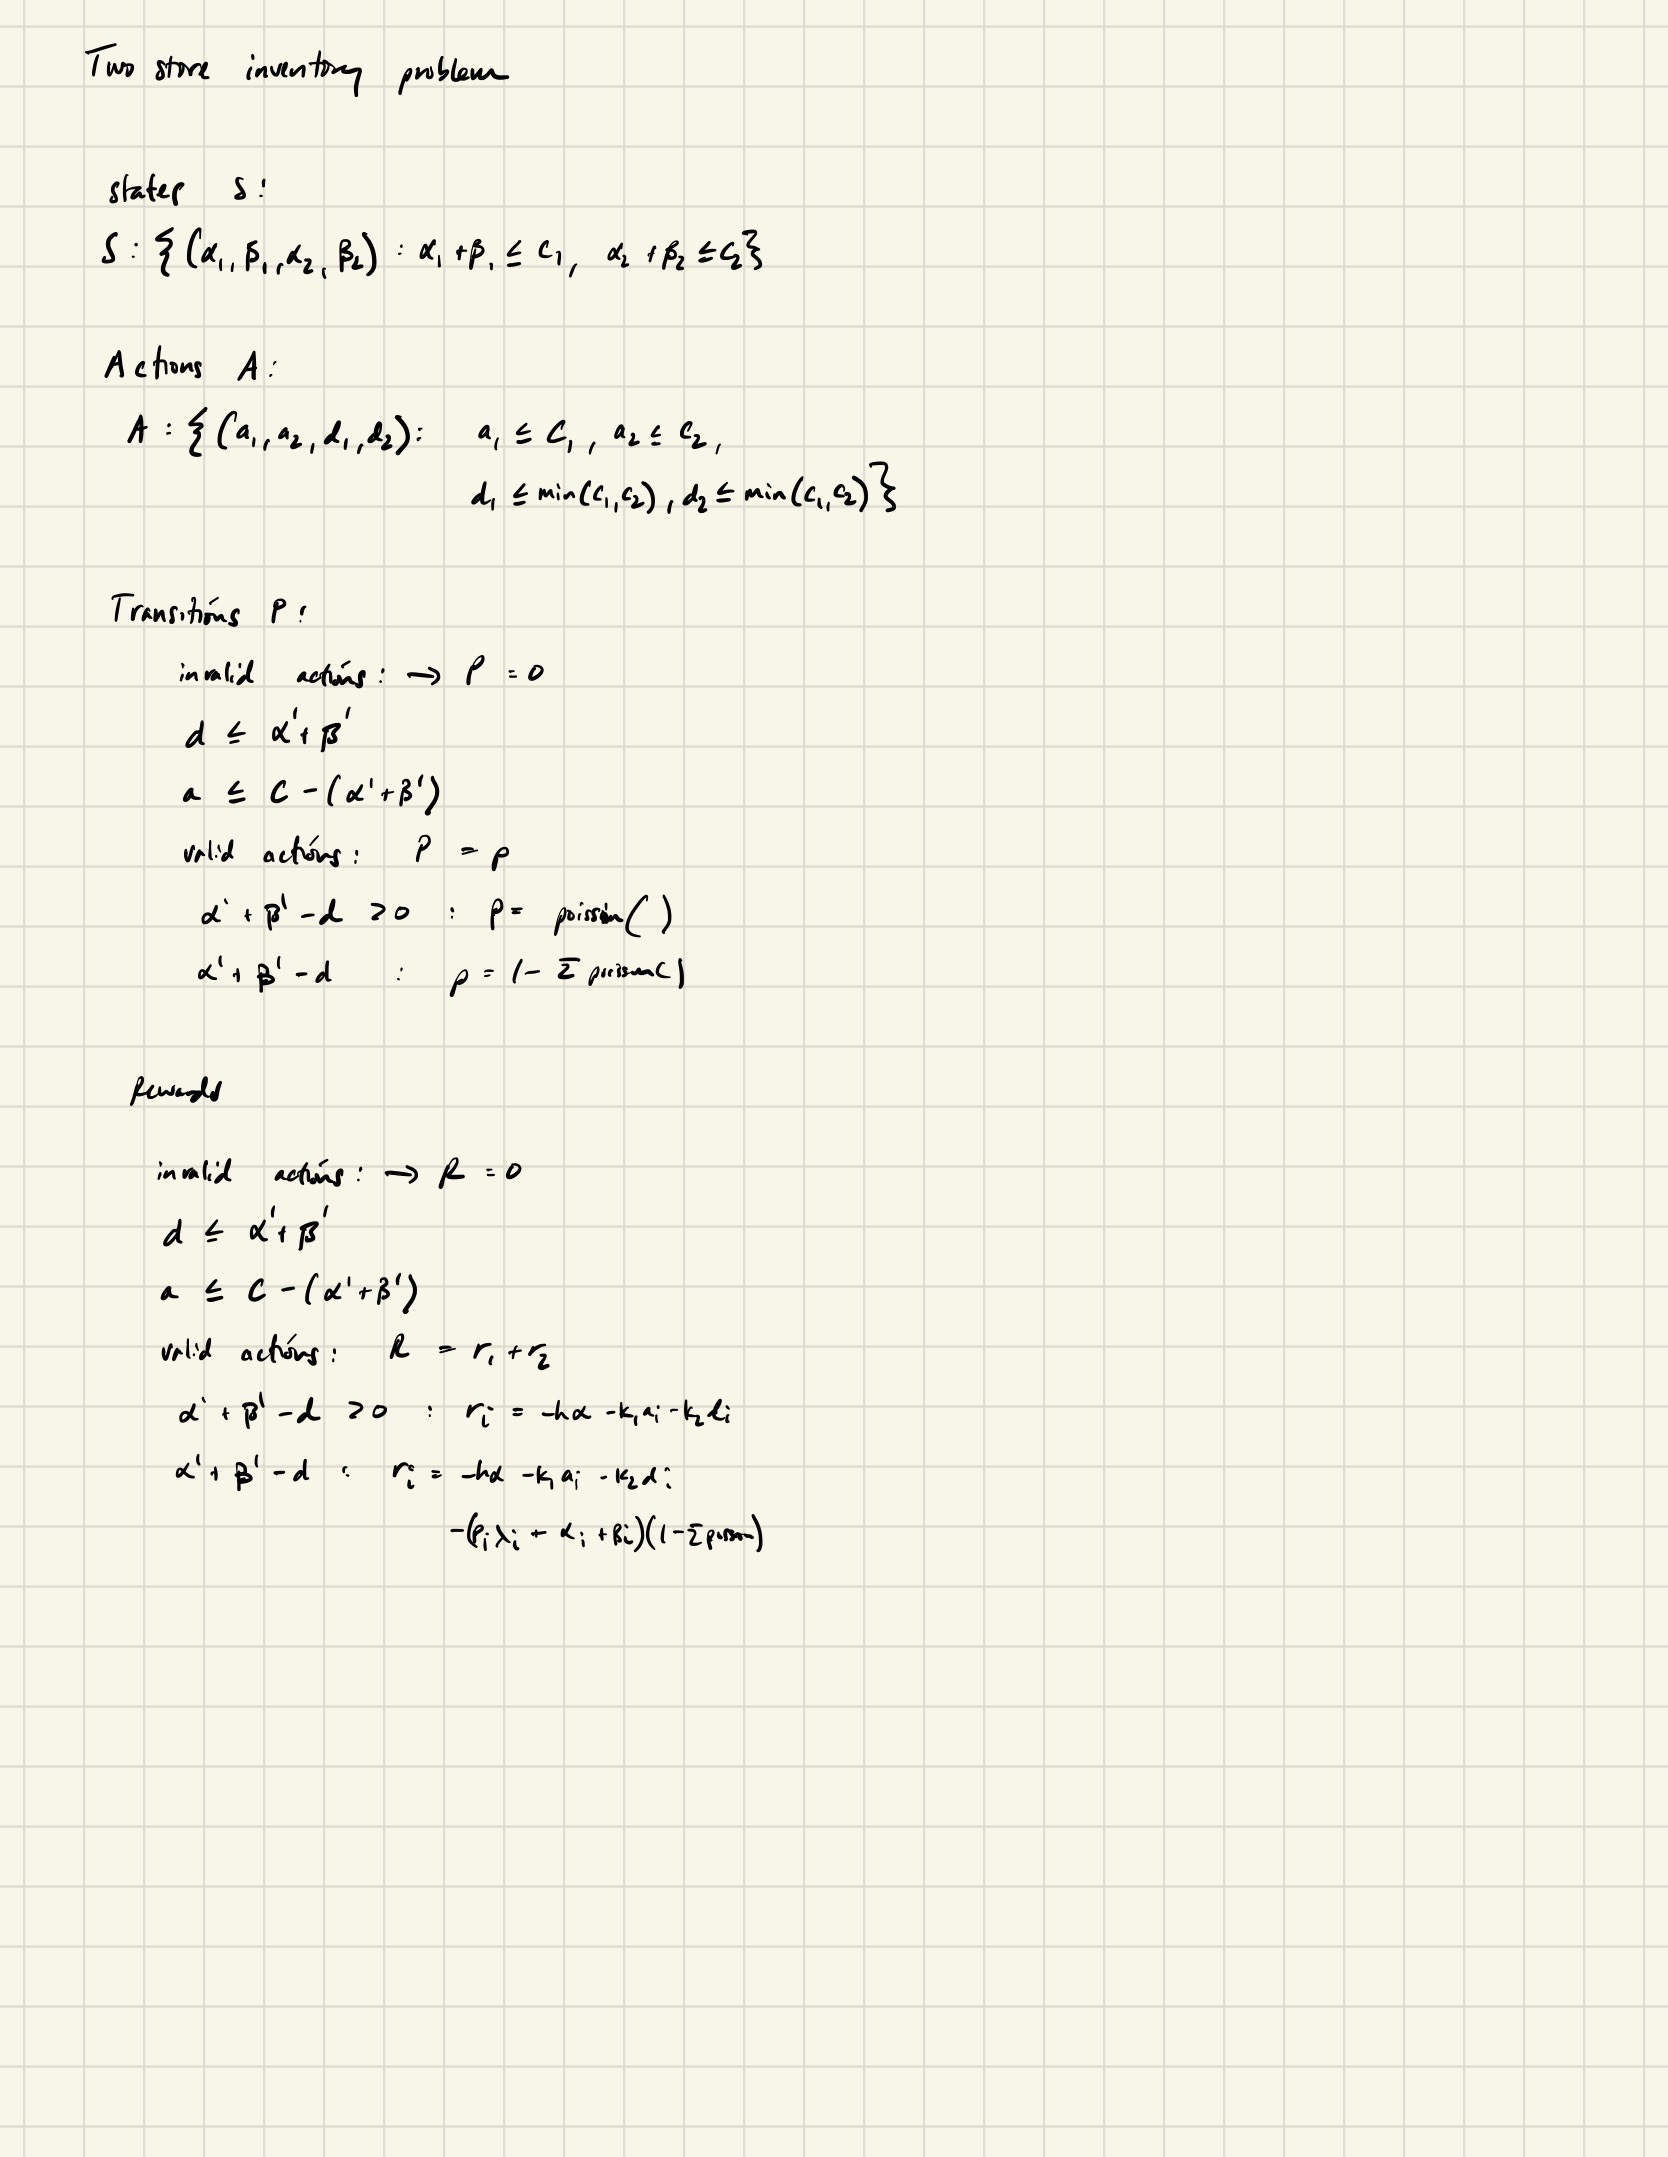
\includegraphics[width=.75\textwidth]{ipad/q4.jpg}
	\caption{Two-store inventory control problem MDP.}
	\label{fig:q4}
\end{figure}


\clearpage


\end{document}
